\documentclass[aps,prl,twocolumn,showpacs,superscriptaddress,10pt]{revtex4-1}  % for review and submission
%\documentclass[aps,twocolumn,floatfix,prl,10pt]{revtex4-1}
%\documentclass[letterpaper,10pt,prl,twocolumn,aps]{revtex4-1}
%\documentclass[aps,preprint,floatfix,prl]{revtex4-1}
\usepackage{amsmath}
\usepackage{amsfonts}
\usepackage{amssymb}
\usepackage{graphicx}
\usepackage{booktabs}
\usepackage{color}
\usepackage{longtable}
\usepackage{array}
\usepackage{amssymb}
\usepackage[usenames,dvipsnames,svgnames,table]{xcolor}

\graphicspath{ {images/}{images/Growth_Rate_Cont_Plots/} }
\newcommand{\bn}{{\boldsymbol{\hat{n}}}}
\newcommand{\bt}{{\boldsymbol{\hat{t}}}}
\newcommand{\bu}{\mathbf{u}}
\newcommand{\grad}{\mathbf{\nabla}}
\newcommand{\del}{\partial}
\newcommand{\hg}{h_g}
\newcommand{\Rey}{\text{R}}
\newcommand{\Ndg}{\tilde{N}_g}
\newcommand{\shreyas}[1]{{\bf (#1)}}
\definecolor{tableShade}{gray}{0.8}

\begin{document}
\title{Linear instability underlying synchronous waving of marine grass in flow}
\author{Ravi Singh}
\affiliation{Brown University, Providence RI 02912 USA}
\author{L. Mahadevan}
\affiliation{Harvard University, Cambridge MA 02138 USA}
\author{Mahesh Bandi\footnote{work performed while visiting Brown University}}
\affiliation{Okinawa Institute of Science and Technology, Okinawa, Japan}
\author{Amala Mahadevan}
\affiliation{Woods Hold Institute of Oceanography, Woods Hole MA USA}
\author{Shreyas Mandre}
\affiliation{Brown University, Providence RI 02912 USA}

\begin{abstract}
%The spontaneous waving of marine grass is thought to be due to a Kelvin-Helmholtz instability resulting from an inflection point in the flow profile. 
%We find that this inflection point is located inside the grass canopy but it does not lead to Kelvin Helmholtz instability which is 
%normally observed in a free shear layer. We also show that the wavelength of coherent vortices scales with the unvegetated water depth, and not with 
%the shear layer thickness as predicted by a theory based on Kelvin-Helmholtz instability. Based on these results, we propose a mechanism for waving 
%marine grass based on the shear instability of the flow above the canopy.

%The spontaneous waving of marine grass is though to be due to a Kelving-helmholtz instability resulting from strong shear near top of grass. On the contrary
%we find that strong velocity shear resulting from vertical discontinuity of drag due to presence of grass does not lead to Kelvin-Helmholtz instability which is 
%normally observed in free shear flows. We also show that wavelength of coherent vortices scales with the unvegetated water depth. Based on these results, 
%we propose an alternative mechanism which attributes waving of marine grass on shear instability of flow above the canopy. 

The spontaneous waving of marine grass is thought to be due to a Kelvin-Helmholtz instability resulting from an inflection point in the flow profile. We find that this inflection point
is located near the tip of grass canopy. Our analysis shows that flow in presence of grass become unstable not only through a mechanism of Kelvin-Helmholtz instability associated with 
inflection point but also through shear instability of flow above grass coupled with the porous flow through grass bed. We further show that in canopy with high submergence ratio
Kelvin-Helmholtz insatbility is damped due to grass drag. 

\end{abstract}
\maketitle

%\section{Introduction}
Sea grasses exhibit rich set of dynamics due to their interaction with the flow of water and can considerably affect surrounding hydrodynamic conditions.
Resulting changes in hydrodynamic conditions can influence number of environmental variables and processes such as 
transport of sediments, contaminants, dissolved oxygen, plant growth and biomass production etc \cite{Fonseca87,Nepf99}. 
The response of flexible grass canopies to steady current in form of large amplitude coherent oscillation, known as mo-nami \cite{AckermanOkubo93}, plays a central role
in the recruitment of microscopic marine organism such as blue mussel larvae \cite{Grizzle96}. The hydrodynamic mechanism underlying monami is the focus of this paper. 

Similar phenomenon of large amplitude coherent oscillation of canopy in atmospheric flow known as ho-nami\cite{Inoue56,Raupach96}, have also been observed.
A crucial difference between the atmospheric and aquatic flow is that the atmospheric flows are essentially unbounded vertically\cite{Vivoni98,Nepf00}. Another major
difference between the two is the considerable difference of stiffness of canopies; terrestrial canopies tend to be much more rigid than aquatic canopies\cite{Vivoni98,Ghisal02}.
Due to these differences between aquatic and marine flow, our analysis of flow in presence of flexible grass in a bounded domain is applicable only to marine canopies. 
  
Existing explanation of monami invokes the existence of strong shear near the top of the canopy \cite{Ghisal02,Raupach96} due to
different amounts of drag experienced by fluid in and above the canopy. This shear layer is assumed to become unstable to coherent vortices through a mechanism similar to 
Kelvin-Helmholtz instability. Influence of these coherent eddies over sea grasses is manifested in their large amplitude synchronous oscillations.


While the shear layer model successfully appears to predict frequency of monami for number of experimental observations, several aspect of existing theory remain unsatisfactory. 
First, linear stability analysis\cite{Raupach96} does not take into account influence of the vegetation and hence is not self consistent. Second, classical free shear flow 
is known to be unstable for all Reynolds number\cite{drazin}, whereas observations in the lab\cite{Ghisal02} and the field\cite{Grizzle96} indicate the existence of a threshold flow speed below which waving is not observed. Finally, the thickness of the free shear layer, defined as the momentum thickness of the boundary layer near the grass tip, is in many cases comparable to the unvegetated layer thickness,
and therefore inconsistent with the assumptions of the free shear layer instability. These drawbacks of existing theory suggest that flow through vegetation requires further investigation for better understanding of the phenomenon.

In this paper we present a mathematical model exhibiting a rich behavior, which is not only consistent within itself, but also with lab experiments and field observations of the threshold.
The synchronous waving may be understood to be arising from the linear instability of a uniform flow over the grass bed. In the limit of a dense grass bed, two distinct unstable modes 
can be asymptotically distinguished, with one of them sharing many characteristics with the Kelvin-Helmholtz instability. In the parameter regime typical of marine grass beds, 
the two modes merge and are indistinguishable.

The drag exerted by the grass bed on the flow is central to the hypothesized mechanism\cite{Ghisal02} of the instability underlying monami because it is directly responsible for 
realizing the shear layer structure of the flow. The flexibility of the grass blades, on the other hand, is considered to merely aid in visualizing the flow structure resulting from 
the instability. It has been demonstrate that the instability and the resulting flow structures are present even when the grass blades are replaced with rigid dowels (citation). 
Therefore, in the interest of deriving the simplest mathematical model for the linear instability, we consider the grass bed to form a rigid structure that exchanges momentum with 
the surrounding fluid but does not deform. Indeed, a more detailed calculation undertaken for terrestrial grass demonstrated\cite{Delangre06} that when the timescale of the instability 
is well-separated from the period of natural oscillations of the grass bed, the flow instability is similar to the 
instability of a shear layer. 

We use a mean field model for the coupling between the flow and the canopy. Drag force exerted by the grass is approximated via a 
continuous body force $\mathbf{f}=-N_g\mathbf{f_d}$ in the fluid momentum balance\cite{Vivoni98,Nepf99,Ghisal02,Delangre04,Delangre06} as
\begin{equation}
\rho \left(\bu_{t}+\bu.\grad\bu \right) = -\grad P+\mu\grad^{2}\bu +\mathbf{f}+\rho\mathbf{g}, \quad \grad\cdot\bu = 0,
\label{navier-stokes}
\end{equation}
where $\mathbf{f_{d}}$ is drag force per unit length of the grass blade, $N_g$ the grass number density per unit area, $\rho$ the fluid density, $\mathbf{u}$ the velocity, 
$P$ the pressure, $\mu$ the turbulent viscosity and $\mathbf{g}$ the acceleration due to gravity. The Reynolds number of the flow on the scale of a grass blade is expected to 
be O($10^2$-$10^3$), and hence the drag force is dominated by form drag, and is modeled 
as $\mathbf{f_{d}}=C_N \rho u_{N}^{2}d\bn + C_{T}\rho u_{T}^{2}d\bt$ where $d$ is average width of grass blade
$C_{N}$ and $C_{T}$ are normal and tangential drag coefficients respectively which are set to zero outside the grass; $\bu_{T}$, $\bu_{N}$ are velocity vector along and
normal to grass while $\bt,\bn$ being unit vector along and normal to grass. We expect $C_T \ll C_N$ and take $C_T=0$ for rest of analysis. In the field, both $C_N \& N_g$ 
vary with distance from the bottom but we do not expect these variation to be central to the mechanism and therefore take $C_N$ \& $N_g$ to be constants. Based on previous experiments\cite{Vivoni98}, we take $C_N \approx 1$.

For consistency of analysis, we calculate the steady flow as a solution of \eqref{navier-stokes}, and examine its linear stability. The steady uniform flow $U(y)$ resulting from solution of \eqref{navier-stokes} is expected to be unstable, leading to coherent eddies underlying monami. Steady state flow driven by constant pressure gradient satisfies
$-{dP}/{dx}+\mu U''(y) +S(y) \rho C_N d N_gU^2=0$, where $S(y)=1$ in the vegetated layer $0<y<\hg$ and $S(y)=0$ in the unvegetated layer $\hg< y< H$. 
The flow in the laboratory experiments is better approximated by zero shear at the bottom ($y=0$) and top ($y=H$) of the fluid layer, as can be seen from the comparison 
between sample solutions and mean flow observed in laboratory experiment shown in Figure \ref{fig:basicflow}. Flow consist of a region of approximately constant velocity
\small$U_g \sim \sqrt{\frac{dP/dx}{\rho C_N dN_g}}$\normalsize arising from balance of drag force with pressure gradient with-in grass and a parabolic velocity 
profile in unvegetated region due to balance of viscous force and pressure gradient. Continuity of flow speed and shear stress at canopy top 
give rise to a boundary layer in the flow profile near the tip of the grass. The boundary layer near the canopy top results from purely local dynamics independent of the influence of the boundaries, and may therefore be identified as a free shear layer\cite{Ghisal02} in the previous explanation of monami. 
In our model, this boundary layer thickness is obtained by balance of viscous force with drag, and matching the shear with that in unvegetated region. This leads to a shear layer 
thickness $\delta = \Rey^{-1/3} \epsilon^{1/3} H$, where $\Ndg = \left[(C_N d H N_g)\right]$, $\Rey=\rho U_0 H/\mu$ is the Reynolds number of the flow, $U_0 = {(dP/dx)~H^2}/{\mu}$ is scale for velocity,
$H$ is half channel width, and $\mu$ the turbulent viscosity. The dependence of the boundary layer thickness on the grass density $N_g$ gives us a way to systematically control it and investigate its effect on the instability mechanism. 
\begin{figure}[htb]
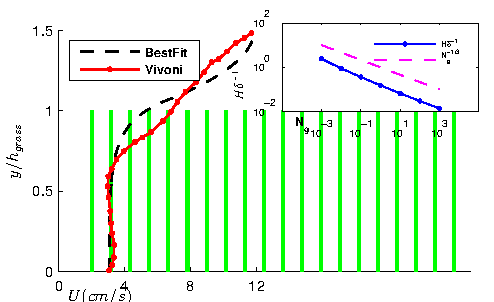
\includegraphics[scale=1]{Grass_Base_Vivoni_shear}
\caption{Base flow profile (left )from the experiment of Vivoni\cite{Vivoni98} (Case-3A (Figure-3.6A) with 330 plants/$m^2$, 6 blades per plant, 
plant height = 16.0$\pm0.2$ and blade width of 0.28cm)
 and it's approximation with $U_0=31cm/s$ and $\delta = 0.2H$ with our model. The model of canopy is shown in the bottom and the variation of shear layer in the inset }
\label{fig:basicflow}
\end{figure}

Considering small perturbations $u, v, p$ about the base profile $U$ and $P$ respectively, equation \eqref{navier-stokes} expanded to linear order in the perturbations yields
\begin{equation}
\begin{split}
\frac{\del u}{\del t}+U\frac{\del u}{\del x}+v\frac{\del U}{\del y} &= -\frac{1}{\rho}\frac{\del p}{\del x}+\frac{\mu}{\rho}\nabla^2u-2S(y) C_{N}dN_{g}Uu, \\
\frac{\del v}{\del  t}+ U\frac{\del v}{\del x} &= -\frac{1}{\rho}\frac{\del p}{\del y}+\frac{\mu}{\rho}\nabla^2v, \hspace{0.3cm} \nabla\cdot\bu=0.
 %\nabla\cdot \bu &= 0
\end{split}
\end{equation}
These equations can be non-dimensionalized using half channel height $H$, velocity $U_0$, and the associated advection time $H/U_0$ . 
We are left with three non-dimensional parameters in the model, viz. the Reynolds number $\Rey$, the vegetation drag parametrized by $\Ndg$, 
and the submergence ratio of the grass $h_g/H$. We also parametrize the grass density through the boundary layer thickness $\delta/H$ to help elucidate the mechanism of the instability. With these scaling, and using a stream function $\psi$ with $u = \psi_{y}, v= -\psi_x$ to satisfy mass balance, we seek a wave solution of the form $\left(u,v,\psi \right)= \left(\hat u, \hat v, \hat\phi \right)e^{ikx+\sigma t}$ to  obtain a modified Orr-Sommerfield equation. The eigenvalue $\sigma$ for a given $k$ provides growth rate and frequency associated with a perturbation of wavelength $2\pi/k$ through the solution of
% \small
\begin{equation}
\begin{split}
\left(D^2 -k^{2} \right)^2\phi &= \Rey \left[ \left({\sigma}+ikU\right) \left(D^2-k^2\right) -ikU_{yy}\right]\phi \\
&+D\left(2R \Ndg S(y) U D \phi\right),
\label{Orr-somerfield}
\end{split}
\end{equation}
where $D=d/dy$, and subject to the boundary conditions $D\phi = D^2\phi = 0$ at $y=\pm 1$. 

\begin{figure}[htb]
\begin{center}
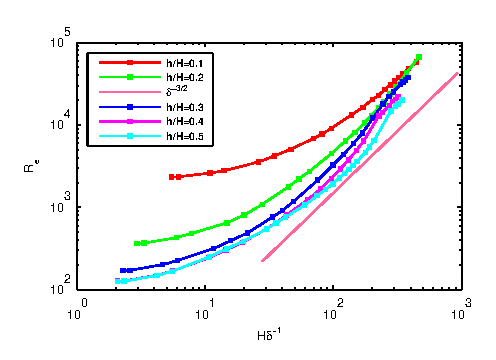
\includegraphics[]{Critical_Re_vs_delta_noshear} \\
\vspace{-6mm} \hspace{-3mm}
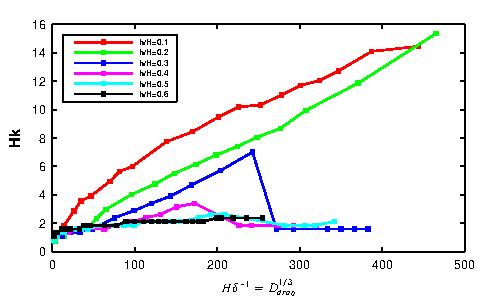
\includegraphics[]{K_vs_shear_width_noshear}
\end{center}
\caption{Critical Reynolds number with flow for different grass height as a function of inverse shear thickness}
\label{Re_vs_delta}
\end{figure}

A threshold in $\Rey$ for the onset of the instability naturally emerges from the solution of \eqref{Orr-somerfield}. The dependence of this critical $\Rey$, and the corresponding fastest growing wavenumber $k$, on the $\delta/H$ and $\hg/H$ is shown in figure \ref{Re_vs_delta}, and compared with experimental observation of the threshold\cite{Ghisal02} without any fitting parameters. 

Comparison of frequency (Im$(\sigma)$) of the fastest growing mode with that of experimental observations of frequencies in the lab scale experiments, for cases where the vegetation was sufficiently dense to be modeled by a continuum drag field, is also shown in Figure \ref{Re_vs_delta}. The observed frequencies are associated with the peaks in velocity spectra, frequency of monami and frequency of vortex passage \shreyas{cite someone}. The deviation of predicted frequency from the observed can be attributed to the various simplification we have made in our model. In a real canopy, the drag coefficients are known to
vary from bottom to tip of the grass blades\cite{Vivoni98,Nepf00}. The turbulent viscosity is also known to vary between the flow of unvegetated region and flow through the canopy. Although these variation
are not central to the mechanism leading to the instability of flow, we believe an improved analysis of flow with these variation in the model might lead to a better agreement between the
observed frequency and the predicted frequency.


\begin{figure*}
\begin{tabular}{cccc}
{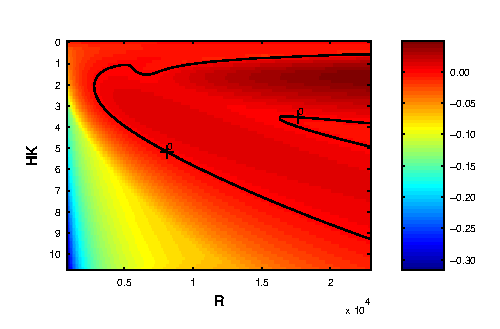
\includegraphics[scale = 0.72]{Set4_dens28_imgsc}} &
{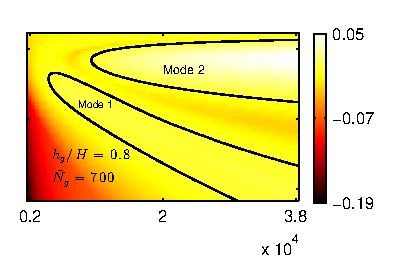
\includegraphics[scale = 0.72]{Set4_dens30_imgsc}} &
{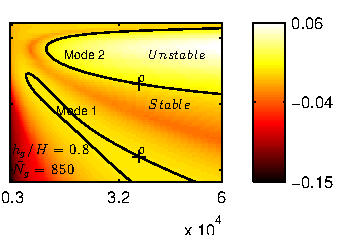
\includegraphics[scale = 0.72]{Set4_dens32_imgsc}} &
{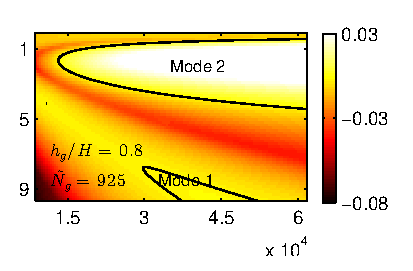
\includegraphics[scale = 0.72]{Set4_dens34_imgsc}} \\
{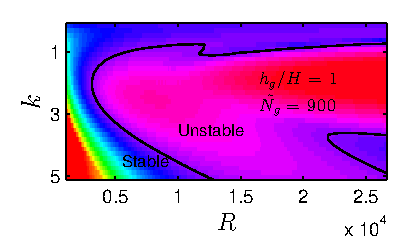
\includegraphics[scale = 0.72]{Set5_dens38_imgsc}} &
{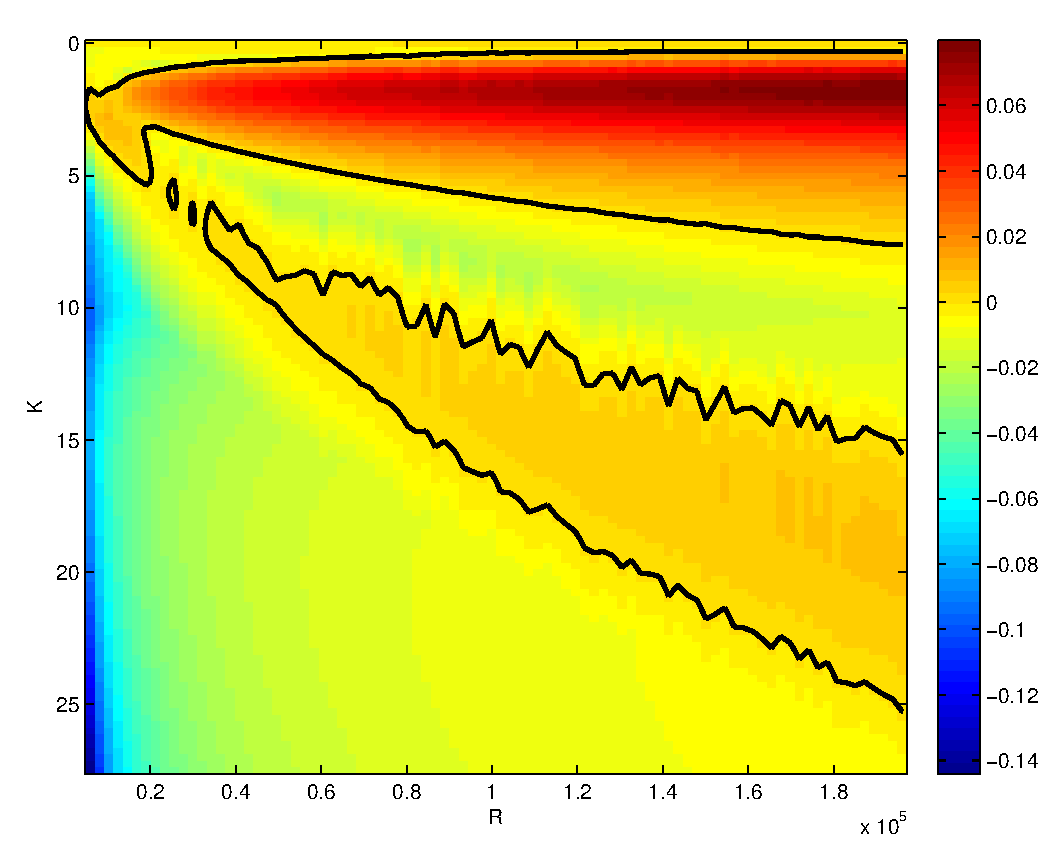
\includegraphics[scale = 0.72]{Set5_dens40_imgsc}} &
{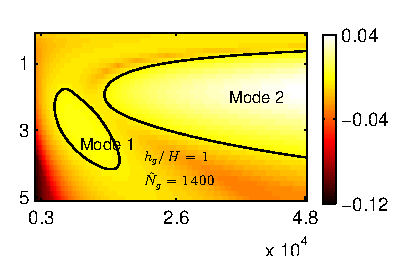
\includegraphics[scale = 0.72]{Set5_dens42_imgsc}} &
{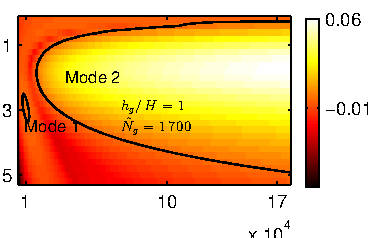
\includegraphics[scale = 0.72]{Set5_dens46_imgsc}} \\
{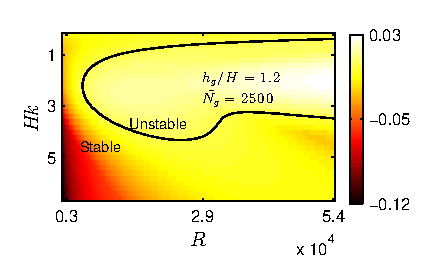
\includegraphics[scale = 0.72]{Set6_dens32_imgsc}} &
{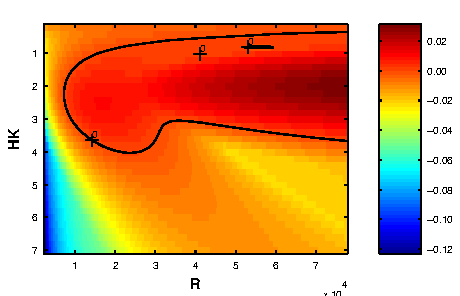
\includegraphics[scale = 0.72]{Set6_dens34_imgsc}} &
{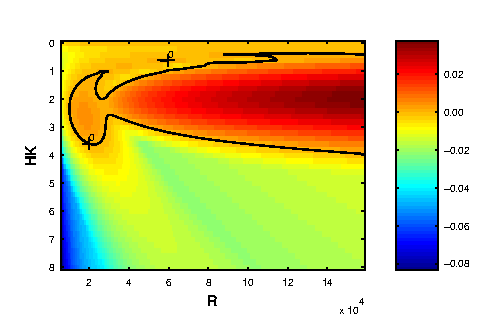
\includegraphics[scale = 0.72]{Set6_dens36_imgsc}} &
{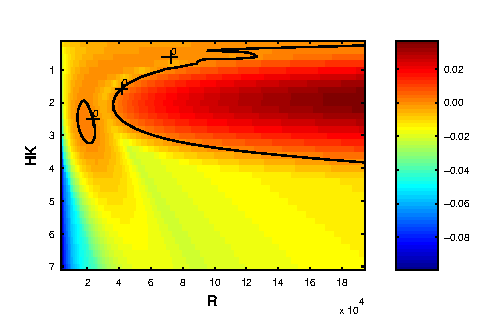
\includegraphics[scale = 0.72]{Set6_dens38_imgsc}}
\end{tabular}

\caption{$Re(\sigma)$ as function of wavenumber and Reynolds number for a given grass number density along with the neutral curve ($Re(\sigma)$=0), for parameters shown in the corresponding panel.  
As $\Re/\epsilon \propto N_g$ increases the unstable region splits into two labeled as ``Mode 1'' and ``Mode 2''. For $N_g$ below
a critical value, the Mode 1 sets the threshold $\Rey$ whereas above the critical $N_{g}$ onset is determined by Mode 2.}
\label{K_Re_sigma_set3}
\end{figure*}

To better understand the mechanism of waving, we consider the behavior of the instability, especially the fastest growing wavenumber, as a function of the vegetation drag, especially as it becomes asymptotically large, i.e. $\Ndg \gg 1$ and $\delta \ll H$. The fastest growing wavenumber first increases proportional to $H/\delta$, but at a critical grass density discontinuously jumps and remains $O(1)$. To aid in explaining the behavior, we show heat maps of Re$(\sigma)$ as a function of $\Rey$ and $kH$, for different $\hg/H$ and $\Ndg$ in figure \ref{K_Re_sigma_set3}. The lowest $\Rey$ on the neutral curve sets the threshold. We observe that as $\Ndg$ increases, the unstable region splits into two. We refer to the unstable region with the higher $k$ as ``Mode 1'', and the one with the lower $k$ as ``Mode 2''. The unstable region for Mode 1, depending on $\hg/H$ either recedes to higher $\Rey$ or shrinks to zero size, as the grass density increases, causing the discontinuity in the most unstable mode.

The distinct asymptotic behavior of the two modes as $\Ndg \gg 1$ allows us to understand the mechanism of the instability. Mode 2 has a threshold $\Rey \sim (\frac{\delta}{H})^{-3/2}$ (or $\Rey \propto \Ndg$) for $k\sim O(1)$, which can be understood by asymptotic analysis of \eqref{Orr-somerfield}.
Noting that for large $\Ndg$, non-dimensional steady flow velocity $U \sim (\Rey \Ndg)^{-1/2}$ inside the grass and $\Rey \gg 1$. So equation \eqref{Orr-somerfield}
can be simplified considerably both with in the grass and above the grass canopy. As $U_{yy}\sim 0$ inside the grass, the equation within the grass simplifies into
$\sigma\left(D^2-k^2\right)\phi = -2{(\Rey\Ndg)^{-1/2}}D^2\phi$ while in the unvegetated region it simplifies to the Rayleigh equation 
$ \left(\sigma+ikU\right) \left(D^2-k^2\right)\phi =  ikU_{yy}\phi$. The mode shape converges to a solution of these equations as $\Rey\gg 1$ and $\Ndg \gg 1$ but $\Rey/\Ndg \sim O(1)$, as shown in figure \ref{Asymptotic_mode}. We interpret this as the instability of an inviscid flow, with the vegetation modeled by a continuum drag field. The only remaining parameter $\Rey \sim (\frac{\delta}{H})^{-3/2}$, therefore sets the threshold.


\begin{figure}[]
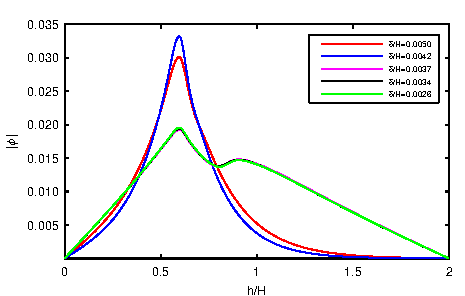
\includegraphics[]{Asymptotic_eig_set3.pdf}
\caption{plot of $|\phi|$ for different shear layer thickness in limit of small shear layer thickness}
\label{Asymptotic_mode}
\end{figure}

On the other hand, Mode 1 asymptotically localizes with a length scale $\delta$ around the grass tip, and exhibits a different asymptotic behavior with $k \sim O(H/\delta)$, and $\Rey \sim (H/\delta)$ (or $\Rey \propto \sqrt{\Ndg}$) at the threshold. This limit can be understood through asymptotically balancing the magnitude of the advection term ($\Rey/\delta^3 \sim \Rey^2 \Ndg $) with that of the viscous term (or the vegetation drag term, which has the same magnitude) in the boundary layer ($\delta^{-4} \sim (\Rey \Ndg)^{4/3}$). The terms balance when $\Rey \sim \sqrt{\Ndg}$, explaining the asymptote. The resulting localization of the the mode structure to a length of $O(\delta)$, is shown in figure \ref{Asymptotic_mode}, supporting this argument.

To conclude, we note that numerical investigation of flow in presence of canopy reveals two distinct modes of flow instability which might lead to monami. The occurrence of these modes for flow instability in a 
canopy depends on its submergence ratio and shear layer thickness. Our analysis predict a threshold criteria characterized by a Reynolds number. The predicted value of threshold Reynolds number agrees well with experimentally observed parameters. Inclusion of variation of drag coefficient along the grass filament might lead to better agreement between the observed and predicted frequency of monami. 

\begin{table*}
\rowcolors{3}{tableShade}{white}  %% start alternating shades from 3rd row
\renewcommand{\arraystretch}{1.4}
 \begin{tabular}{l|c|c|c}
			& Kelvin-Helmholtz 				& Mode 1 		& Mode 2 \\ \hline
 Base velocity profile 	& $U(y) = U_0 \tanh(y/\delta)$			& \multicolumn{2}{c}{$-{dP}/{dx}+\mu U''(y) +S(y) \rho C_N d N_gU^2=0$} \\
 Domain 		& $-\infty < y < \infty$			& \multicolumn{2}{c}{$-1<y<1$} \\
 Inflection point	& exists at $y=0$				& \multicolumn{2}{c}{$U''(y)$ discontinuous at $y=\hg$} \\
 Shear layer thickness	& $\delta$					& \multicolumn{2}{c}{$\delta \sim  H\left[({\rho U_0 H}/\mu) (C_N d N_g H)\right]^{-1/3}$} \\
 Linearized dynamics	& Inviscid Rayleigh's equation			& \multicolumn{2}{c}{Equation \eqref{Orr-somerfield}} \\
 Critical parameters	& none						& $\Rey$, $\delta/H$ 	& $\Rey \delta^{3/2}$ \\
 Most unstable $k$ as $\delta \to 0$	& $\propto \delta^{-1}$		& $\propto \delta^{-1}$	& $O(1)$ \\
 Mode localized?	& yes, near $y=0$				& ~~~~yes, near $y=\hg$~~~~			& no
 \end{tabular}
 \caption{Comparison between Kelvin-Helmholtz instability and the two modes presented here.}
\end{table*}

\bibliography{Grass}{}
\bibliographystyle{plain}
\end{document}
